\section{Overview of Actario}
\label{sec:overview}

\subsection{Programming in Actario}

Actario is a Coq framework for defining and verifying actor-based
systems. A typical workflow using Actario is as follows.
\begin{enumerate}
\item Describe an actor system using types and notations defined in the framework.
\item Specify and verify desired properties of the system.
\item Extract the Erlang version of the system using the code extraction mechanism of Coq.
\end{enumerate}
Note that Actario does not provide a dedicated language for describing
actor systems.  The framework offers a set of Coq vocabularies (types
and notations described in Section~\ref{sec:typesandnotations}) for
that purpose.


\paragraph{Example: Recursive Factorial System}
We use a simple example to illustrate a system description in Actario.
Figure~\ref{coq:fact} shows the definition of an actor system that
implements the continuation-passing style factorial function adapted
from \cite{Agha:1986aa}.  In this definition, the function
\lstinline|factorial_system| sets up a system that initially consists
of a single factorial actor whose behavior is defined as
\lstinline|factorial_behv|.  The actor can receive a tuple of a
natural number and the name of a \emph{customer} actor
(\lstinline|cust|) that is intended to receive the result.  If the
first component of tuple is more than zero, \textit{i.e.}, it matches
the successor pattern \lstinline|S n|, the actor creates a new
continuation actor (\lstinline|cont|) and recursively sends itself a
pair of \lstinline|n| and \lstinline|cont|.  The behavior of
continuation actors is specified as \lstinline|factorial_cont_behv|.

\begin{figure}[t]
\begin{lstlisting}[style=small]
Definition factorial_cont_behv (val : nat)
                               (cust : name) :=
  receive (fun msg =>
    match msg with
     | nat_msg arg => cust ! nat_msg (val * arg);
                      become empty_behv
     | _ => become empty_behv
    end).

CoFixpoint factorial_behv :=
  receive (fun msg =>
    match msg with
     | tuple_msg (nat_msg 0) (name_msg cust) =>
       cust ! nat_msg 1;
       become factorial_behv
     | tuple_msg (nat_msg (S n)) (name_msg cust) =>
       cont <- new (factorial_cont_behv (S n) cust);
       me <- self;
       me ! tuple_msg (nat_msg n) (name_msg cont);
       become factorial_behv
     | _ => become factorial_behv
    end).

Definition factorial_system (n : nat) (cust : name) :=
  init "factorial" (
    x <- new factorial_behv;
    x ! tuple_msg (nat_msg n) (name_msg cust);
    become empty_behv
  ).
\end{lstlisting}
\caption{Recursive Factorial System in Actario}\label{coq:fact}
\end{figure}

%% \begin{figure}[t]
%% \centering
%% 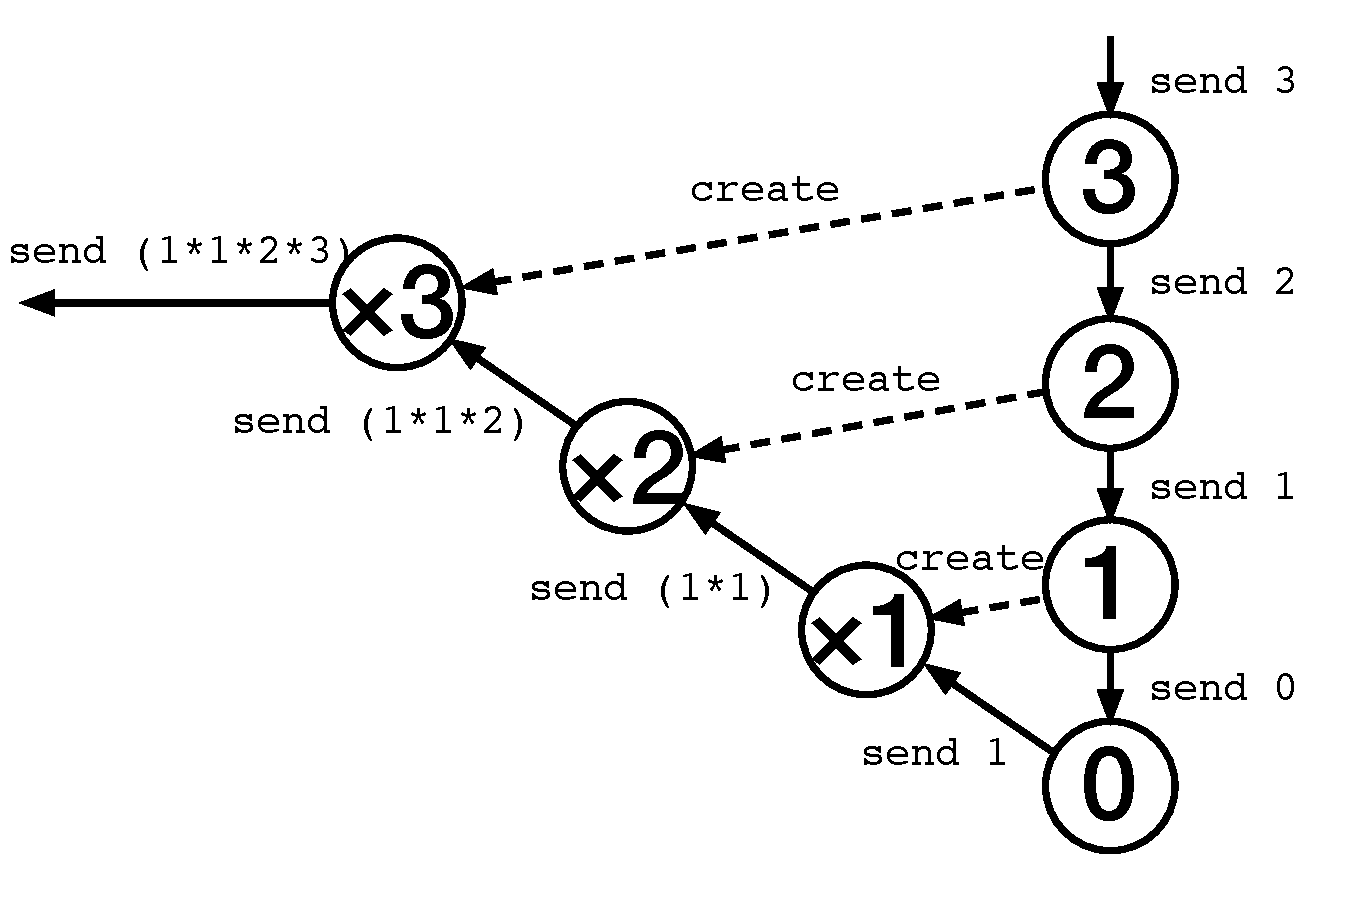
\includegraphics[width=8cm]{./images/fact.pdf}
%% \caption{Recursive Factorial}\label{fig:fact}
%% \end{figure}


\begin{figure}
\begin{lstlisting}
Inductive message : Set :=
 | empty_msg : message
 | name_msg : name -> message
 | str_msg : string -> message
 | nat_msg : nat -> message
 | bool_msg : bool -> message
 | tuple_msg : message -> message -> message.
\end{lstlisting}
\caption{Message Type}\label{coq:message}
\end{figure}

\begin{figure}
\begin{lstlisting}
CoInductive actions : Type :=
 | new : behavior -> (name -> actions) -> actions
 | send : name -> message -> actions -> actions
 | self : (name -> actions) -> actions
 | become : behavior -> actions
with behavior : Type :=
 | receive : (message -> actions) -> behavior.
\end{lstlisting}
\caption{Types for Actions and Behaviors}\label{coq:actions}
\end{figure}

\subsection{Types and Notations}\label{sec:typesandnotations}

\subsubsection{Types}

Figure~\ref{coq:message} shows the inductively defined type of messages delivered
among actors, each of whose constructors corresponds to a kind of
messages.  In the current version of Actario, a message may be empty,
an actor name, a value of basic types (Boolean, natural number or
string), or a tuple of two messages.

Figure~\ref{coq:actions} defines two mutually coinductive types:
\lstinline|actions| and \lstinline|behavior|. They specify sequences
of actions performed by actors and behaviors of actors respectively.
Each constructor of \lstinline|actions| corresponds to a single action embedded in
an action sequence as follows.
\begin{description}

\item[\texttt{new} \(b\) \(f\)] creates a new actor with initial
  behavior \(b\) and applies \(f\) to the name of the created
  actor. Then continues to the action sequence that \(f\) returns.

\item[\texttt{send} \(n\) \(m\) \(\alpha\)] sends message \(m\) to the
  actor with name \(n\) and then continues to action sequence
  \(\alpha\).

\item[\texttt{self} \(f\)] retrieves the name of the actor that executes this
  action and applies \(f\) to it. Then continues to the action sequence
  that \(f\) returns.

\item[\texttt{become} \(b\)] sets \(b\) as the next behavior of the
  actor that executes this action. This action should end an action
  sequence.
\end{description}

In the Actor model, an actor persists indefinitely. Thus, as shown in
Figure~\ref{coq:fact}, that a behavior may have \lstinline|become|
actions that specify itself or other behaviors eventually recurring to
the original one.  The reason for using \lstinline|CoFixpoint| and
defining \lstinline|actions| and \lstinline|behavior| coinductively is
to model such behaviors.


\subsubsection{Notations}

In addition to the types defined above, Actario provides a collection
of notations (syntactic sugaring) described in
Figure~\ref{coq:notation}.  Using the notations, we can write actor
behaviors intuitively without being complicated by CPS.
Figure~\ref{fig:notationexample} compares the descriptions of a simple
action sequence without/with the notations.

\begin{figure}
\begin{lstlisting}
Notation ``n '<-' 'new' behv ; cont'' :=
    (new behv (fun n => cont))
    (at level 0, cont at level 10).
Notation ``n '!' m ';' a'' :=
    (send n m a) (at level 0, a at level 10).
Notation ``me '<-' 'self' ';' cont'' :=
    (self (fun me => cont))
    (at level 0, cont at level 10).
\end{lstlisting}
\caption{Notations for Actions}\label{coq:notation}
\end{figure}

\begin{figure}\centering
\begin{minipage}{0.2\textwidth}\centering
\begin{lstlisting}[frame=single]
new $b$ (fun x =>
self (fun s =>
send x (name_msg s)
(become $b'$)))
\end{lstlisting}
(a) without notations
\end{minipage}
\hspace*{3ex}
\begin{minipage}{0.2\textwidth}\centering
\begin{lstlisting}[frame=single]
x <- new $b$;
s <- self;
x ! (name_msg s);
become $b'$
\end{lstlisting}
(b) with notations
\end{minipage}
\caption{Example Use of Notations}\label{fig:notationexample}
\end{figure}
